\documentclass[acmsmall,nonacm]{acmart}

% acmart already provides amsmath/amsthm/amssymb, booktabs, graphicx,
% xcolor, array, and hyperref; add only what it does not.
\usepackage{listings}
\usepackage{tikz}
\usetikzlibrary{arrows.meta,positioning,calc}
\usepackage{makecell}
\usepackage{float}
\setlength{\headheight}{18.48402pt} % satisfy fancyhdr's required header height (acmart)
\addtolength{\topmargin}{-5.48402pt}
\setlength{\emergencystretch}{3em} % absorb overfull lines from unbreakable inline code

\settopmatter{printacmref=false}   % preprint: suppress the ACM reference block
\raggedbottom                      % figure-heavy: let slack fall to page bottom,
                                   % not stretch above pinned [H] figures

%% Theorem environment (acmart `acmplain` style; `invariant` italic)
\theoremstyle{acmplain}
\newtheorem{invariant}{Invariant}
%% Inline code
\newcommand{\code}[1]{\texttt{#1}}

%% Java listings
\definecolor{codegray}{gray}{0.45}
\definecolor{codeblue}{rgb}{0.13,0.29,0.53}
\definecolor{codebg}{rgb}{0.97,0.97,0.97}
\lstdefinestyle{java}{
  language=Java,
  basicstyle=\small\ttfamily,
  columns=fullflexible,
  keepspaces=true,
  keywordstyle=\color{codeblue}\bfseries,
  commentstyle=\color{codegray}\itshape,
  stringstyle=\color{codegray},
  backgroundcolor=\color{codebg},
  frame=single,
  framesep=4pt,
  rulecolor=\color{black!15},
  xleftmargin=6pt,
  xrightmargin=6pt,
  breaklines=true,
  breakatwhitespace=true,
  showstringspaces=false,
  tabsize=2,
  numbers=none,
  morekeywords={abstract,implements,extends,interface,class,new,return,
                public,private,protected,static,final,void,String,boolean,
                int,Object,Override,System,out,println,@link,@part},
}
\lstset{style=java}

%% Kotlin listings
\lstdefinestyle{kotlin}{
  language=,
  basicstyle=\small\ttfamily,
  columns=fullflexible,
  keepspaces=true,
  keywordstyle=\color{codeblue}\bfseries,
  commentstyle=\color{codegray}\itshape,
  stringstyle=\color{codegray},
  backgroundcolor=\color{codebg},
  frame=single,
  framesep=4pt,
  rulecolor=\color{black!15},
  xleftmargin=6pt,
  xrightmargin=6pt,
  breaklines=true,
  breakatwhitespace=true,
  showstringspaces=false,
  tabsize=2,
  numbers=none,
  morekeywords={fun,val,var,class,interface,override,by,abstract,open,
                private,public,protected,String,Unit,Any,return,if,else},
}


\begin{document}

\title{Interface-Scoped Dispatch:\texorpdfstring{\\}{ }Independent Components with \texorpdfstring{$\boldsymbol{O(1)}$}{O(1)} Self-Calls}

\author{R. Scott McKinney}
\affiliation{\institution{Manifold Systems}\country{USA}}
\email{scott@manifold.systems}
\renewcommand{\shortauthors}{McKinney}

\begin{abstract}
A longstanding tenet of object-oriented design is to favor composition over implementation inheritance. But to fully move
off the inheritance crutch, a general composition model is needed that does not sacrifice the qualities of conventional
composition that make it favorable: independent runtime components and arbitrary composition. At the same time it must retain
the defining property of inheritance: open recursion. These three properties together define such a model.

No general-purpose language satisfies all three. Existing approaches fall into two modes: forwarding-based composition keeps
independent components and arbitrary topologies but forfeits open recursion, since a component's self-calls never reach
overriding composites; trait-based composition recovers open recursion by fusing components into a single compile-time object,
forfeiting their independence and dynamic composition. Research models reach past both modes but still sacrifice independence,
arbitrary composition, or performance.

We present Parts, a general composition model that maintains these properties without compromise. Realized as a compiler
plugin for Java 8–26, Parts reconciles the properties of conventional object composition with open recursion. The enabling
mechanism, interface-scoped dispatch (ISD), assigns composite identity per interface at construction. The dispatch cost
is $O(1)$, empirically equivalent to a vtable call.
\end{abstract}

\maketitle

%% ─────────────────────────────────────────────────────────────────────────────
\section{Introduction}
\label{sec:intro}
%% ─────────────────────────────────────────────────────────────────────────────

Object composition is the standard prescription for structuring behavior from reusable components~\cite{gamma1994}. Newer
mainstream languages (Rust, Swift, and Go) took this route to avoid the hazards of implementation inheritance, primarily
fragile base classes and tight coupling to superclass internals. But avoiding those hazards with object composition alone
introduced new ones.

Abandoning implementation inheritance isn't wrong, but inheritance has at least one quality worth keeping: open recursion.
The behavior is particularly useful with interface-based object composition where a component's interface self-calls can
reach composite overrides. But none of these languages provide this capability.

This paper proposes a general composition model that does. Our model cleanly reconciles the essential properties
of object composition: \emph{independent components} (late-bound objects supplied at construction) and \emph{arbitrary composition}
(unrestricted delegation topologies), with \emph{open recursion} (self-calls through the composite). Existing composition
models typically circle these properties, never achieving all three (Section~\ref{sec:related}).

The conventional object composition of modern composition-based languages differs in implementation but comes down to basic forwarding.
Some, like Rust and Swift, require manual forwarding; others, via constructs such as Kotlin's by clause~\cite{kotlin}, forward
automatically. All supply independent components under arbitrary composition, but none have open recursion,
because plain objects do not preserve references to the forwarding composites required to resolve self-calls. This
is the \emph{Object Schizophrenia} problem~\cite{sekharaiah2002,kniesel2000}.

Trait composition (Scala \code{with}~\cite{odersky2005}, mixins~\cite{bracha1990}) inverts the trade. Self-calls dispatch
through \code{this} in the linearized class, so composite overrides are visible. But traits are fused into the hierarchy
at compile time, resulting in a single runtime object; component independence and runtime defined composition structure
are lost. Composition is static and limited to a single-rooted, merged hierarchy.

Several research projects (Section~\ref{sec:related}) have produced delegation-based composition models that achieve independent
components with open recursion, but only within limited topologies, not the full gamut supported in conventional object composition
(Section~\ref{subsec:topologies}). Equally critical, these models tend to introduce auxiliary machinery to support open recursion,
resulting in additional implementation complexity and runtime overhead that make them less practical.

With \code{@part} and \code{@link}, \emph{Parts} satisfies all three properties. A \emph{part} (a class annotated with \code{@part})
is an independent component supplied at construction. A \emph{composite} (a class with one or more fields annotated
with \code{@link}) delegates the interfaces declared on the linked fields to parts. When a composite is constructed, the compiler
plugin wires composite identity into each part per delegated interface, enabling self-calls in the part to dispatch through
the composite. A link field accepts any implementation of its declared interface: forwarding therefore works with ordinary
objects, while part objects additionally provide open recursion. Parts thus subsumes forwarding, enabling both forwarding
with plain objects and delegation with parts in the same composite.

The enabling mechanism is \emph{interface-scoped dispatch} (ISD): assigning composite identity per interface at construction
makes open recursion possible under arbitrary composition. Because dispatch is interface-scoped, self-calls retain $O(1)$
dispatch cost.

The core contributions are:

\begin{itemize}
  \item \textbf{Parts}: a model for object composition in which
        components are independent runtime objects, composable arbitrarily
        under partial delegation, with self-calls dispatching through
        the composite and interface contracts statically enforced.
        The model is defined over standard interface hierarchies with a central
        dispatch invariant (Invariant~\ref{prop:dispatch}) and
        composite-scoped encapsulation (\code{@internal}).
  \item \textbf{Interface-scoped dispatch (ISD)}: the mechanism that assigns
        composite identity per interface at construction, enabling
        open recursion under arbitrary composition via partial
        delegation (where a composite claims a proper subset of a part's
        interfaces).
  \item \textbf{An implementation}: a compiler plugin for
        Java 8--26 realizing the model with $O(1)$ self-dispatch cost, with open-source
        release~\cite{mckinney2026} and IDE integration.
\end{itemize}

%% ─────────────────────────────────────────────────────────────────────────────
\section{Overview}
%% ─────────────────────────────────────────────────────────────────────────────

Consider a minimal example that shows \code{@part} and \code{@link} working in a concrete single-rooted composite.

\begin{lstlisting}
interface Actor {
  void takeAction();
  void attack();
}

@part class Hero implements Actor {
  public void takeAction() { attack(); }
  public void attack() { println("Swing club!"); }
}

class Wizard implements Actor {
  @link Actor actor;
  Wizard(Actor actor) { this.actor = actor; }
  @Override public void attack() { println("Cast spell!"); }
}

new Wizard(new Hero()).takeAction(); // "Cast spell!"
\end{lstlisting}

When \code{Wizard} is constructed, the compiler wires \code{Hero}'s
composite identity for \code{Actor} to \code{Wizard}. A call to
\code{takeAction()} dispatches to \code{Hero.takeAction()}, and the self-call
\code{attack()} within it dispatches back through \code{Wizard}, invoking
\code{Wizard.attack()}, not \code{Hero.attack()}.

This is the decorator pattern with one addition: the wrapped object's self-call
routes back through the composite. A plain decorator would forward
\code{takeAction()} to the \code{Hero}, whose \code{attack()} call would stay on
\code{Hero} (``Swing club!''), losing the override.

Because the link field accepts any \code{Actor} at construction
time, the part is a real late-bound object, not fused into the class
hierarchy. A different \code{Actor} implementation can be substituted
without changing \code{Wizard}.

Interface contracts are enforced at compile time: the link field has
type \code{Actor}, and the compiler verifies that \code{Wizard}
implements the delegated interface. A raw part may not escape the
composite dispatch path: passing or assigning \code{this} as the concrete
part type is a compile error; interface or Object types are required.

This example is single-rooted: \code{Wizard} is the sole composite
for \code{Hero}, and one composite identity suffices. The following
section exposes the limit of the single-identity model and the per-interface
generalization that resolves it.

%% ─────────────────────────────────────────────────────────────────────────────
\section{The Model}
\label{sec:model}
%% ─────────────────────────────────────────────────────────────────────────────

\subsection{Motivating example}

The following example shows a part whose interfaces are rooted at different
composites. \code{Hero} implements both \code{Combatant} and \code{Actor},
and two wrappers decorate it: a \code{Wizard} changes how it fights
(\code{Combatant}), while a \code{Demon} partially possesses it, seizing its name
and will (\code{Actor}) but leaving its trained combat untouched. As in the
overview, the wrapped hero's self-calls route back through the wrappers; now two
wrappers claim different interfaces of the same part. So from a single \code{Hero}
instance, \code{attack()} must route through \code{Wizard} and \code{name()}
through \code{Demon}; a single composite identity cannot serve both. Assigning a
separate composite identity per interface resolves this.
Figures~\ref{fig:dag-diagram} and~\ref{fig:dag-listing} show the structure.

\begin{figure}[H]
\centering
\begin{tikzpicture}[
  cls/.style={
    draw, rectangle, rounded corners=3pt,
    minimum width=5.5cm, inner sep=8pt,
    align=center, font=\small
  },
  lnk/.style={->, >=Stealth, semithick},
]
\node[cls] (wp)
  {\textbf{Hero}\\[3pt]
   \textit{implements Combatant, Actor}};

\node[cls, below=2cm of wp] (lw)
  {\textbf{Wizard}\\[3pt]
   \textit{implements Combatant, Actor}};

\node[cls, below=2cm of lw] (app)
  {\textbf{Demon}\\[3pt]
   \textit{implements Actor}};

%% Wizard @link -> Hero
\draw[lnk] ([xshift=-12pt]lw.north)
  -- node[left,  font=\scriptsize\ttfamily] {@link Combatant}
  ([xshift=-12pt]wp.south);
\draw[lnk] ([xshift=12pt]lw.north)
  -- node[right, font=\scriptsize\ttfamily] {@link Actor}
  ([xshift=12pt]wp.south);

%% Demon @link -> Wizard
\draw[lnk] (app.north)
  -- node[right, font=\scriptsize\ttfamily] {@link Actor}
  (lw.south);

%% Dispatch root annotations
\node[font=\scriptsize\itshape, text=gray, right=0.5cm of lw, anchor=west]
  {Combatant root};
\node[font=\scriptsize\itshape, text=gray, right=0.5cm of app, anchor=west]
  {Actor root};
\end{tikzpicture}
\caption{Composition structure. Arrows show link fields labeled
by the delegated interface. \code{Wizard} is the root for
\code{Combatant} dispatch; \code{Demon} is the root for \code{Actor} dispatch.}
\label{fig:dag-diagram}
\Description{A three-class composition. Hero implements Combatant and
Actor. Wizard links both interfaces of Hero and is the Combatant root.
Demon links the Actor interface of Wizard and is the Actor root.}
\end{figure}

\begin{figure}[H]
\begin{lstlisting}
interface Combatant {
  void attack();
}
interface Actor {
  String name();
  void takeAction();
}

@part class Hero implements Combatant, Actor {
  public void attack() { println("Swing club!"); }
  public String name() { return "Milo"; }
  public void takeAction() {
    out.print(name() + " acts: ");  // Actor dispatch
    attack();                       // Combatant dispatch
  }
}

@part class Wizard implements Combatant, Actor {
  @link Combatant combatant;
  @link Actor actor;
  Wizard(Hero h) { this.combatant = h; this.actor = h; }
  public void attack() { println("Cast spell!"); }
}

class Demon implements Actor {
  @link Actor actor;
  Demon(Actor a) { this.actor = a; }
  public String name() { return "Diablo"; }
}

Wizard wizard = new Wizard(new Hero());
Demon demon = new Demon(wizard);
demon.takeAction();
// Actor dispatch rooted at Demon
// Combatant dispatch rooted at Wizard
// prints:  Diablo acts: Cast spell!
\end{lstlisting}
\caption{Composition with multiple composite roots per part.
\code{Hero} carries distinct composite identities for \code{Combatant}
(rooted at \code{Wizard}) and \code{Actor} (rooted at \code{Demon}).}
\label{fig:dag-listing}
\Description{Java source listing of the Hero, Wizard, and Demon
composition, showing distinct composite roots per interface.}
\end{figure}

\subsection{Definitions}

We define Parts over a standard typed object model where
classes implement interfaces and method dispatch is defined by the receiver's
runtime type.

A \emph{part} is a class annotated with \code{@part} and implements one or
more interfaces. A \emph{link} is an ordinary field annotated with \code{@link} typed
as an interface implemented by the enclosing class. The interface is delegated to the link's value, assigned at construction.
Links are implicitly \code{private} and \code{final} (explicit modifiers are redundant).
A class containing one or more links is a \emph{composite}, it nominally implements
every interface its links claim. The \emph{delegation surface} of a part is its interface hierarchy,
excluding any interface marked \code{@internal} in its \code{implements} clause.

When a composite links an interface to a part, the part is directly wired to the composite;
it records a \emph{composite identity}: a reference to the composite statically indexed by the interface.
The part's self-calls route through the composite indexed by the interface of the called method. The enabling mechanism
is \emph{interface-scoped dispatch} (ISD).

A part may itself contain link fields, in which case composite identity
propagates transitively. When such a part is wired to an outer composite, that
composite becomes the dispatch root for each interface it claims throughout the
delegation chain, while interfaces it does not claim retain the roots
established by inner composites. This \emph{transitive propagation} traverses
part links only: it terminates at any non-part link, a regular object whose
self-calls remain local to the delegate. A composition may thus freely mix parts
and non-part delegates, with no interaction between them.

Composites must also resolve \emph{diamonds}. When a composite has multiple links that share a common
interface, the authoritative link must be chosen via \code{@link(share=I.class)} at one of the link sites.
This determines the leg of the diamond the linking composite forwards through. The other links wire the
composite normally: self-calls on the shared interface always dispatch through the linking composite to the
component on the authoritative leg.

Two practical extensions, composite-scoped encapsulation (\code{@internal})
and abstract parts with deferred linkage (\code{asLink()}), are defined
and implemented (Section~\ref{sec:impl}).

\paragraph{Dispatch rule.}
Traditional object-oriented dispatch resolves a call through the receiver's
object identity:
\[ \text{call } m() \text{ on } o \;\longrightarrow\; \mathit{vtable}(o,\, m) \]
Interface-scoped dispatch replaces the single object identity with a
per-interface composite identity. A self-call $m()$ in part $P$ where
$m \in I$ resolves through the composite identity for $I$:
\[ \text{self-call } m() \in I \text{ in } P \;\longrightarrow\;
   \$\mathit{selves}_P[I].m() \]
For self-calls within a part's methods, the dispatch triple is
\emph{(part, interface, method)} rather than the conventional
\emph{(object, method)}.
Figure~\ref{fig:dispatch-comparison} contrasts this per-interface routing with a single shared composite identity.
This is \emph{open recursion}: a method's self-calls late-bind to the
most-derived receiver. Here the receiver resolves from the interface of the self-call. Forwarding is the closed case: a
component's self-calls stay in the component, and the composite never enters
the recursion.

\begin{figure}[H]
\centering
\begin{tikzpicture}[
  >=Stealth,
  cbox/.style={draw, rectangle, minimum width=2.6cm, minimum height=0.8cm,
               inner sep=4pt, align=center, font=\small},
  svbox/.style={draw=black!45, fill=gray!15, rectangle, minimum width=2.6cm,
                inner sep=2pt, align=center, font=\scriptsize\ttfamily},
  sbox/.style={draw=black!45, fill=gray!15, rectangle, minimum width=2.6cm,
               inner sep=2pt, align=center, font=\scriptsize\ttfamily},
  darr/.style={->, black!45, semithick},
  lbl/.style={font=\scriptsize\itshape, text=black!55},
]

%%====================================================================
%% LEFT PANEL -- Object Scoped
%%====================================================================
\node[font=\bfseries] at (-3.0, 2.0) {Object Scoped};
\node[lbl, text=black!75] at (-3.0, 1.5)
  {\textit{self-call} $m \in I_1$ inside $P$};

\node[cbox] (PL) at (-3.0, 0.8) {$P$ \ impl $I_1$,\,$I_2$};
\node[sbox, below=0pt of PL, minimum height=0.74cm] (BL) {\texttt{\$self}};
\node[cbox] (C1L) at (-3.0, -1.7) {$C_1$ \ impl $I_1$,\,$I_2$};
\node[cbox] (C2L) at (-3.0, -3.6) {$C_2$ \ impl $I_1$,\,$I_2$};

\draw[darr] (C1L.north) -- (BL.south)
  node[midway, right, xshift=3pt, lbl] {delegate $I_1$,\,$I_2$};
\draw[darr] (C2L.north) -- (C1L.south)
  node[midway, right, xshift=3pt, lbl] {delegate $I_2$};

\draw[{Circle[fill=red!80!black, scale=0.7]}->, red!80!black, thick, dashed]
  (BL.west)
  .. controls ($(BL.west)+(-1.1, 0)$) and ($(C2L.west)+(-1.1, 0)$) ..
  (C2L.west)
  node[pos=0.5, anchor=east, xshift=-4pt, lbl, align=right,
       text=red!70!black]
    {dispatch $I_1$ \ $\times$};

\node[font=\small, text=red!80!black, below=0.2cm of C2L, align=center]
  {wrong dispatch target for $I_1$};

%%====================================================================
%% DIVIDER
%%====================================================================
\draw[black!20, dashed] (0, 2.4) -- (0, -4.8);

%%====================================================================
%% RIGHT PANEL -- Interface Scoped
%%====================================================================
\node[font=\bfseries] at (3.0, 2.0) {Interface Scoped};
\node[lbl, text=black!75] at (3.0, 1.5)
  {\textit{self-call} $m \in I_1$ inside $P$};

\node[cbox] (PR) at (3.0, 0.8) {$P$ \ impl $I_1$,\,$I_2$};
\node[svbox, below=0pt of PR, minimum height=0.74cm] (BR)
  {\texttt{\$selves[$I_1$]}\\[1pt]\texttt{\$selves[$I_2$]}};
\node[cbox] (C1R) at (3.0, -1.7) {$C_1$ \ impl $I_1$,\,$I_2$};
\node[cbox] (C2R) at (3.0, -3.6) {$C_2$ \ impl $I_1$,\,$I_2$};

\draw[darr] (C1R.north) -- (BR.south)
  node[midway, left, xshift=-3pt, lbl] {delegate $I_1$,\,$I_2$};
\draw[darr] (C2R.north) -- (C1R.south)
  node[midway, left, xshift=-3pt, lbl] {delegate $I_2$};

\coordinate (slotI1) at ($(BR.north east)!0.27!(BR.south east)$);
\coordinate (slotI2) at ($(BR.north east)!0.73!(BR.south east)$);

\draw[{Circle[fill=black, scale=0.7]}->, black, thick]
  (slotI1)
  .. controls ($(slotI1)+(0.85, 0)$) and ($(C1R.east)+(0.85, 0)$) ..
  (C1R.east)
  node[pos=0.5, anchor=west, xshift=4pt, lbl, text=black!80]
    {dispatch $I_1$ \ $\checkmark$};

\draw[{Circle[fill=black!30, scale=0.7]}->, black!30, semithick]
  (slotI2)
  .. controls ($(slotI2)+(1.3, 0)$) and ($(C2R.east)+(1.3, 0)$) ..
  (C2R.east)
  node[pos=0.5, anchor=west, xshift=4pt, lbl, text=black!35]
    {dispatch $I_2$};

\end{tikzpicture}
\caption{Object-scoped vs.\ interface-scoped dispatch. In both panels $C_2$
(impl~$I_1$,\,$I_2$) delegates only $I_2$ to $C_1$ (impl~$I_1$,\,$I_2$), which delegates
both interfaces to part $P$.
\emph{Left:} a self-call $m() \in I_1$ inside $P$ routes through
\texttt{\$self\,=\,$C_2$}, the wrong composite for $I_1$.
\emph{Right:} \texttt{\$selves[$I_1$]} routes to $C_1$;
\texttt{\$selves[$I_2$]} routes to $C_2$; each self-call reaches its
correct composite root.}
\label{fig:dispatch-comparison}
\Description{Side-by-side comparison of object-scoped versus interface-scoped
dispatch. Left panel shows a single identity slot routing an $I_1$ self-call
to the wrong composite. Right panel shows per-interface slots routing each
self-call to its correct composite root.}
\end{figure}

\begin{invariant}
\label{prop:dispatch}
For any part $P$ in a delegation chain for interface $I$ rooted at
composite $C$: a self-call \code{this.m()} within $P$ where $m \in I$
dispatches to $C$.
\end{invariant}

This invariant presumes each interface has a single composite root. The model
maintains this precondition for every composition it admits but does not
statically enforce it; the lone exception is treated in Section~\ref{sec:limitations}.

The invariant is established by construction. When composite $C$ establishes
a link to part $P$ for interface $I$, the plugin-generated
\code{\$linkPartToSelf} sets $\$\mathit{selves}_P[I] \leftarrow C$ and
recurses into $P$'s own links, propagating $C$'s identity for each interface
$C$ claims and leaving all other slots unchanged. Each interface of a part resolves
through a single \code{\$selves} slot. Wiring an outer composite that claims
$I$ re-roots this slot to that composite and leaves the slots for interfaces it
does not claim unchanged, so the slot holds exactly one root at any time and
stabilizes once the outermost composite claiming $I$ is wired; $C$ denotes that
final root. Each write occurs during the wiring composite's construction. Wiring happens solely
as link field assignment, and the plugin enforces \code{final} on link
fields, so writes are confined to construction: the \code{\$selves} slots are never
written after the outermost composite claiming $I$ is constructed.

Visibility follows from safe publication: once the composite root is safely published, the
Java Memory Model guarantees that any thread observing it sees all writes that
happened-before publication, the wired slots included. The role of \code{final}
here is write-confinement, not the JMM's final-field freeze: array-element writes
are not covered by freeze semantics, so the guarantee rests on write-confinement
together with safe publication of the root, not on the finality of the slots.

Self-calls in $P$ where $m \in I$ are rewritten by
the plugin to \code{((I)\,\$selves[IDX\_I]).m()}; when $m$ belongs to multiple
interfaces (the diamond case), $I$ is determined at compile time by diamond
resolution (Section~\ref{sec:impl}). For self-calls through the delegation surface, there is no code path in a
part method that dispatches through anything other than the indexed
slot. Because the slot holds $C$ once the composition is constructed and is not
written thereafter, the invariant holds at every point a self-call can execute.
Before wiring, each slot is initialized to \code{this}; an unwired part
dispatches on itself, consistent with standard object-oriented dispatch. In this
initial state, the invariant holds trivially.
A full mechanized proof in a Featherweight Java subset is a natural direction
for follow-on work (Section~\ref{sec:futurework}).

\subsection{Arbitrary Composition}
\label{subsec:topologies}

Parts supports behaviorally acyclic graphs where nodes may be parts, composites, or ordinary objects, and
edges are link fields. Each edge connects a composite to a component through the interface the link claims.

Partial delegation permits a composite to claim only the interfaces it needs from a part's
delegation surface, leaving the remaining interfaces for other composites to claim. This freedom
gives rise to the four composition topology primitives shown in Figure~\ref{fig:topologies}
and classified over two dimensions: the number of roots a part maintains and the number of sources the composition has.
A root is an outermost node claiming one or more interfaces of a part's delegation surface; a source is a node with no incoming
link edges.

\begin{enumerate}
\item[(a)] \textbf{Single-root, single-source.}
Composite $A$ implements $I_1, I_2$ and delegates both to $B$, which
implements both directly. $A$'s links claim all of $B$'s delegation surface,
so $B$ has one root, $A$, for both interfaces, and one source. This is the
topology typical of decorator chains.

\item[(b)] \textbf{Multi-root, single-source.}
Composite $A$ implements $I_1, I_2$ and delegates only $I_1$ to $B$,
which implements $I_1, I_2$ directly. Because $A$ does not claim $B$'s $I_2$,
$I_1$ is rooted in $A$, while $I_2$ is rooted in $B$: one source, two roots.
$A$ and $B$ in turn may delegate their free interfaces to separate components that
participate in another subgraph that likewise decomposes into one of
these four topologies. The motivating example discussed previously
(Figure~\ref{fig:dag-diagram}) is an instance of this topology combined with (a)
where $B$ delegates both its $I_1$ and $I_2$ to another part,
propagating $A$ and $B$ as the part's roots for $I_1$ and $I_2$.

\item[(c)] \textbf{Multi-root, multi-source.}
Component $C$ implements $I_1$ and $I_2$, where $A$ claims $I_1$ and
$B$ claims $I_2$. As in (b), $C$ has different roots for its two
interfaces, but here $A$ and $B$ are independent sources. This echoes
subject-oriented programming's independent \emph{subjects}, composed
with no single subject designated as owner (Section~\ref{sec:related}).
Figure~\ref{fig:topology-c-listing} exercises this directly.

\item[(d)] \textbf{Cyclic, multi-root, sourceless.}
Composite $A$ implements $I_1, I_2$ and delegates $I_1$ to $B$, which
implements $I_1, I_2$ and delegates $I_2$ back to $A$. Such cycles are
permitted when delegation through the cycle is behaviorally terminal
because each traversal proceeds through a distinct interface: $I_1$
is rooted in $A$, and $I_2$ is rooted in $B$. Cycles over nondistinct interfaces
are rejected (Section~\ref{sec:impl}).
\end{enumerate}

Each of the four topologies illustrated takes its reduced form using as few nodes and edges as possible while retaining
the essential properties that make the topology distinct. Topologies (a) and (b) each have a single source, but (b) is multi-root;
(c) is multi-root and multi-source; (d) is multi-root and sourceless. Topology (d) is structurally cyclic but behaviorally
acyclic over distinct interfaces.

These four are exhaustive over the two dimensions. Of the six combinations the dimensions admit, two cannot occur: a
single-rooted part forces a single source, and a sourceless graph is necessarily multi-root. This leaves (a)–(d).

These topologies provide a basis for verifying whether a composition model supports arbitrary composition: does its treatment
of open recursion remain correct under arbitrary extensions of each topology?

Another set of labeled edges may be drawn onto the structural delegation graph to form a second graph in which each part
is connected to the composites claiming its interfaces, determined by following the delegation edges backwards along each
interface of the part's delegation surface to the outermost composite claiming the interface. This derived identity graph
reveals what open recursion under arbitrary composition requires: composite identity assigned per interface and wired at
construction.

In all four cases, for each delegated interface, a part acquires the identity of the composite claiming that interface,
independent of where execution enters the composition. Invariant~\ref{prop:dispatch} holds independently for each interface.

Ordinary object composition already admits these topologies freely; nothing prevents the use of partial delegation to
build compositions mirroring these structures. The differentiator is open recursion: without it, a component's
self-calls remain effectively static and do not reach composite overrides. Parts fills this crucial gap comprehensively
via interface-scoped identity, ensuring self-calls dispatch correctly regardless of how the composition is structured.

\begin{figure}[H]
\centering
\begin{minipage}[t]{0.19\linewidth}
\centering
\begin{tikzpicture}[
  cls/.style={draw, rectangle, rounded corners=2pt, minimum width=1.5cm,
              minimum height=0.55cm, inner sep=2pt, align=center, font=\scriptsize},
lnk/.style={->, >=Stealth, semithick},
lbl/.style={font=\tiny\ttfamily},
]
\node[cls] (B) at (0,1.0) {$B$ \\ impl $I_1,I_2$};
\node[cls] (A) at (0,-0.3) {$A$ \\ impl $I_1,I_2$};
\draw[lnk] (A.north) -- (B.south) node[midway, right, lbl] {$I_1,I_2$};
\end{tikzpicture}\\[3pt]
{\scriptsize (a) single-root, single-source\\ $I_1,I_2$ root: $A$}
\end{minipage}
\hfill
\begin{minipage}[t]{0.19\linewidth}
\centering
\begin{tikzpicture}[
  cls/.style={draw, rectangle, rounded corners=2pt, minimum width=1.5cm,
              minimum height=0.55cm, inner sep=2pt, align=center, font=\scriptsize},
lnk/.style={->, >=Stealth, semithick},
lbl/.style={font=\tiny\ttfamily},
]
\node[cls] (B) at (0,1.0) {$B$ \\ impl $I_1,I_2$};
\node[cls] (A) at (0,-0.3) {$A$ \\ impl $I_1,I_2$};
\draw[lnk] (A.north) -- (B.south) node[midway, right, lbl] {$I_1$};
\end{tikzpicture}\\[3pt]
{\scriptsize (b) multi-root, single-source\\ $I_1$ root: $A$;\ $I_2$ root: $B$}
\end{minipage}
\hfill
\begin{minipage}[t]{0.27\linewidth}
\centering
\begin{tikzpicture}[
cls/.style={draw, rectangle, rounded corners=2pt, minimum width=1.5cm,
              minimum height=0.55cm, inner sep=2pt, align=center, font=\scriptsize},
lnk/.style={->, >=Stealth, semithick},
lbl/.style={font=\tiny\ttfamily},
]
\node[cls] (C) at (0,1.0) {$C$ \\ impl $I_1,I_2$};
\node[cls] (A) at (-0.95,-0.5) {$A$ \\ impl $I_1$};
\node[cls] (B) at (0.95,-0.5) {$B$ \\ impl $I_2$};
\draw[lnk] (A.north) -- (C.south west) node[midway, left, lbl] {$I_1$};
\draw[lnk] (B.north) -- (C.south east) node[midway, right, lbl] {$I_2$};
\end{tikzpicture}\\[3pt]
{\scriptsize (c) multi-root, multi-source\\
$I_1$ root: $A$;\ $I_2$ root: $B$}
\end{minipage}
\hfill
\begin{minipage}[t]{0.19\linewidth}
\centering
\begin{tikzpicture}[
  cls/.style={draw, rectangle, rounded corners=2pt, minimum width=1.5cm,
              minimum height=0.55cm, inner sep=2pt, align=center, font=\scriptsize},
  lnk/.style={->, >=Stealth, semithick},
  lbl/.style={font=\tiny\ttfamily},
]
\useasboundingbox (-1.45,-0.75) rectangle (1.45,1.4);
\node[cls] (B) at (0,1.0) {$B$ \\ impl $I_1,I_2$};
\node[cls] (A) at (0,-0.4) {$A$ \\ impl $I_1,I_2$};
\draw[lnk] (A.east) to[out=25, in=-25] node[pos=0.5, right, lbl] {$I_1$} (B.east);
\draw[lnk] (B.west) to[out=205, in=155] node[pos=0.5, left, lbl] {$I_2$} (A.west);
\end{tikzpicture}\\[3pt]
{\scriptsize (d) multi-root, sourceless,\\ $I_1$ root: $A$;\ $I_2$ root: $B$}
\end{minipage}
\caption{The four primary composition topologies under partial delegation.
Arrows point from a delegating composite to the part it links.
(a) and (b) have a single source; (c) has two sources; (d) is sourceless.}
\label{fig:topologies}
\Description{Four diagrams of composition topology primitives. (a) Two classes, A and
B, with A delegating both interfaces to B, rooted at A. (b) Two classes, A and B,
where A delegates only I1 to B, meaning I1 is rooted at A while I2 is rooted at B.
(c) Two independent classes A and B, with no edge between them, each delegating a
different interface directly to the same class C, so C has two roots with no common ancestor.
(d) A cycle between classes A and B, where A delegates I1 to B and B delegates I2
back to A, forming a two-node cycle where each interface resolves to its respective root.}
\end{figure}

\begin{figure}[H]
\begin{lstlisting}
interface Actor { void takeAction(); int timeLimit(); }
interface Combatant { int strengthLevel(); }

@part class BasicHero implements Actor, Combatant {
  private int elapsedTime = 11;
  public void takeAction() { println("Attack with strength: " + strengthLevel()); }
  public int timeLimit() { return 10; }
  public int strengthLevel() { return outOfTime() ? 0 : 8; }
  private boolean outOfTime() { return elapsedTime > timeLimit(); }
}
class PaidSubscriber implements Actor {
  @link Actor actor;
  PaidSubscriber(Actor actor) { this.actor = actor; }
  public int timeLimit() { return 100; }
}
class SuperSoldierAddon implements Combatant {
  @link Combatant combatant;
  SuperSoldierAddon(Combatant combatant) { this.combatant = combatant; }
  public int strengthLevel() { return combatant.strengthLevel() * 10; }
}
BasicHero basicHero = new BasicHero();
PaidSubscriber subscriber = new PaidSubscriber(basicHero);
SuperSoldierAddon addon = new SuperSoldierAddon(basicHero);
subscriber.takeAction(); // reaches SuperSoldierAddon's strengthLevel()
// PaidSubscriber and SuperSoldierAddon hold no reference to each other.
// prints: Attack with strength: 80
\end{lstlisting}
\caption{Topology (c): two independent composites, \code{PaidSubscriber} and
\code{SuperSoldierAddon}, claim different interfaces of the same \code{BasicHero} with no
common composite. The call \code{subscriber.takeAction()} reaches self-calls
through the respective roots: \code{strengthLevel()} through
\code{SuperSoldierAddon} and \code{timeLimit()} through \code{PaidSubscriber}.}
\label{fig:topology-c-listing}
\Description{Java source listing showing two unrelated composites, PaidSubscriber
and SuperSoldierAddon, each linking a different interface of the same BasicHero part, with
no reference between them. The call to takeAction reaches strengthLevel through
SuperSoldierAddon and timeLimit through PaidSubscriber.}
\end{figure}

%% ─────────────────────────────────────────────────────────────────────────────
\section{Implementation}
\label{sec:impl}
%% ─────────────────────────────────────────────────────────────────────────────

The implementation is a \texttt{javac} plugin operating on the compiler's AST
during two phases. In \textsc{enter}, the plugin generates structural
scaffolding: the \code{\$selves} composite identity array and
\code{\$linkPartToSelf} wiring method for each part, delegation
forwarding method for each composite class, and (for abstract parts) the
\code{\$Impl} subclass and \code{asLink()} factories. In \textsc{analyze},
after type resolution, self-calls in part methods are rewritten,
link field assignments are rewritten to invoke wiring, and
\code{@internal} visibility is enforced. No bytecode manipulation is performed;
all transformation is at the AST level and subject to standard type checking.

\subsection{Part Transformation}

Each part holds a \code{\$selves} array whose compile-time-determined ordinals
cover the part's interfaces.

\begin{lstlisting}[language={},style=java]
private final Object[] $selves = {this, ..., this};
// after wiring: $selves[IDX_I] = composite identity for interface I
\end{lstlisting}

Before wiring, every \code{\$selves} slot holds \code{this}, so the part
dispatches on itself. Wired at link assignment via \code{\$linkPartToSelf}, dispatch routes
through the composite defining the link. \code{\$linkPartToSelf} updates each
relevant slot and recurses through link fields in the part whose delegation
surface includes the interface being propagated, with cycle detection at each
assignment.

Within a part method, every call \code{this.m(args)} where \code{m} is declared in interface $I$ is rewritten to:

\begin{lstlisting}
((I) $selves[IDX_I]).m(args)
\end{lstlisting}

The cast ensures interface method invocation via the \code{invokeinterface} instruction, which guarantees the composite
receiver will itself route the call correctly within its runtime implementation, regardless of indirection such as with
bridge methods.

The ordinal \code{IDX\_I} is assigned per part over its own
delegation surface, so it is local to that class: the rewritten self-calls and
the generated \code{\$linkPartToSelf} both reside in the part and share its
indexing, and no index agreement across separately-compiled classes is required.

\subsection{Composite Transformation}

A composite implements every interface claimed by its links. For each method of
a claimed interface that the composite does not implement directly, the plugin
generates a delegating method that forwards through the corresponding
link field:

\begin{lstlisting}
R m(args) { return link.m(args); }
\end{lstlisting}

When two links share an interface, the forwarders for the
shared methods route through the authoritative link
(Section~\ref{sec:model}). The non-authoritative link's part need not hold
the authoritative instance: its \code{\$selves} slot for the shared interface
points at the composite, so the shared methods dispatch through the composite
to the authoritative link. Where a part implements the shared interface
directly, that implementation is overridden by delegation, with no instance
shared.

In composite classes, each link field assignment \code{this.link = expr}
is rewritten to invoke \code{\$linkPartToSelf}, propagating the composite
identity into the part. An \code{instanceof} check guards the call so
that non-part assignments pass through unchanged.

\subsection{Abstract Part Support}

A part may be abstract, deferring some interface methods to the
composite. Linking an abstract part obligates the composite to implement those
methods or to be declared abstract. When enforceable at compile time: the plugin
generates a delegating method for every interface method the part implements and
none for a method it leaves abstract, so a concrete composite is missing exactly
those methods and \texttt{javac} rejects it unless they are supplied directly.
This is the compositional analog of the rule that a concrete class must implement
its inherited abstract methods.

To make an abstract part instantiable for linking, the compiler generates a
private \code{\$Impl} subclass whose stubs throw \code{DelegationLinkageError},
and an \code{asLink()} factory per constructor:

\begin{lstlisting}
private static final class $Impl extends Foo {
  $Impl(/* ctor args */) { super(/* ctor args */); }
  @Override public T m(Params p) {
    throw new DelegationLinkageError(
      "abstract method called on an unlinked part");
  }
}
public static Foo asLink(/* ctor args */) { return new $Impl(/* same */); }
\end{lstlisting}

Once wired, the stubs are unreachable for a compile-time configured abstract part:
self-calls dispatch through \code{\$selves} to the composite, whose implementation
the compile-time obligation guarantees. The stubs remain for the runtime configured
case when the linking composite does not override the part's abstract methods, and
as a runtime guard for an \code{asLink()} instance invoked before the part is wired.

\subsection{Default Methods}
\label{subsec:default}

If left unmitigated, a default method runs with the part as receiver,
rather than the composite, when neither the composite nor the part overrides it,
resulting in incorrect self-call dispatch.

No bytecode instruction directly invokes a default with a receiver other
than the current \code{this}, but a method handle bound to an \code{invokedynamic}
call site works around this limitation. When a part does not override a default, the plugin
generates an override that invokes the interface's default implementation through
such a site, with the receiver taken from the interface's slot in \code{\$selves},
so the default's self-calls dispatch through that receiver. An explicit
\code{I.super.m()} in part code is rewritten the same way.

\begin{lstlisting}
interface Foo {
  void bar();
  // default self-calls bar()
  default void foo(P p) { bar(); }
}

@part class FooPart implements Foo {
  public void bar() { ... }

  // generated
  // calls Foo.super.foo() with composite in $selves as receiver
  // Foo's bar() self-call dispatches through the composite
  public void foo(P p) {
    invokedynamic Foo::foo((Foo) $selves[IDX_Foo], p);
  }
}
\end{lstlisting}

The site's bootstrap links it once to a fixed target (the default implementation),
with the receiver as its only varying argument. Being
monomorphic, it is inlined by the JIT to the same type of array-indexed
invocation as in Section~\ref{sec:eval}.

\subsection{Safety Guarantees}
\label{subsec:safety}

\paragraph{Cycle detection.}
If a part is wired to itself directly or transitively over the same interface,
\code{De\-le\-ga\-tion\-Link\-age\-Er\-ror} is thrown at assignment time during
the recursive \code{\$linkPartToSelf()} call.

\paragraph{Deferred method access.}
The obligation that a wired composite implement an abstract part's deferred methods is enforced at compile time; an \code{asLink()} instance invoked before wiring throws \code{DelegationLinkageError} from the \code{\$Impl} stub, the compositional analog of \code{AbstractMethodError}.

\paragraph{\code{@internal} enforcement.}
\code{@internal} may annotate an interface method or an interface type literal
in a class's \code{implements} clause, with distinct effects. A marked method has its calls confined to the composite, the intent behind \code{protected} in implementation inheritance, but more cleanly scoped for composition. A marked
interface type literal in a class's \code{implements}
clause removes that interface from the class's delegation surface: no composite may claim it via a link field.

\paragraph{Self-preservation.}
Inside a part, \code{this} use is guarded. Field access, private calls,
and callbacks through the part's own link fields (the compositional
analog of \code{super}) are all permitted. Passing or assigning \code{this} as
the concrete part type is not: that is a compile error, since a caller
holding the bare part could invoke methods outside the composite dispatch
path and violate Invariant~\ref{prop:dispatch}. The only \code{this} that can leave is therefore either interface-typed or
\code{Object}-typed: resolving to the composite claiming the interface or the
part itself. A client receiving it reaches the composite's overrides.

%% ─────────────────────────────────────────────────────────────────────────────
\section{Evaluation}
\label{sec:eval}
%% ─────────────────────────────────────────────────────────────────────────────

\subsection{Dispatch Performance}

The dispatch path for a self-call through a composite is:
\begin{enumerate}
  \item Load \code{\$selves[IDX\_I]}, an array-indexed load with compile-time
        constant index
  \item Cast to $I$
  \item \code{invokeinterface m}, standard JVM virtual dispatch
\end{enumerate}

This is $O(1)$. The parallel to vtable dispatch is direct: a vtable
call is an indexed slot load followed by an indirect call. Call sites in typical
compositions are monomorphic or bimorphic, the JIT's most aggressively optimized
scenarios. Composite dispatch adds at most one additional virtual dispatch over
direct delegation.

\paragraph{Benchmark.}
We verify this empirically using JMH~\cite{jmh} in average-time mode.
Each scenario calls \code{compute()} through a composite root at chain
depth $d$ (1--6). The \emph{baseline} traverses $d$ \code{@link} delegation
hops to a leaf that returns directly, with no self-call. The \emph{concrete}
variant traverses the same hops but the leaf issues a self-call
(\code{\$selves[IDX\_I].scale()}) from a concrete part method,
dispatching through the composite root. The \emph{default} variant issues the
same self-call from an inherited interface default method the leaf does not
override, routed through the generated \code{invokedynamic} override of
Section~\ref{subsec:default}. The delta (concrete minus baseline) isolates the cost of the self-call
dispatch mechanism alone. All runs: 10 JVM forks,
5 warmup iterations, 10 measurement iterations per fork (100 data points per
cell); errors are $\pm$\,half-width of the 99.9\% confidence interval.
A separate single-dispatch calibration run (\code{invokeinterface}
on a monomorphic call site, same harness) yields 0.43\,ns/op; the delta
values in Table~\ref{tab:bench} are therefore roughly 1--2$\times$ a single virtual
dispatch.

\paragraph{Choice of baseline.}
The delta is measured against Parts's own forwarding path, which is the right
baseline: that path is semantically equivalent to Kotlin \code{by} and Lombok
\code{@Delegate} (Section~\ref{sec:related}), so the delta prices exactly the
self-call routing those mechanisms cannot express, against their own dispatch
cost. A cross-system benchmark against other composition models would price
differences in implementation strategy rather than the self-call dispatch this
delta isolates, so that comparison is analytic (Section~\ref{sec:related}).

\begin{table}[htbp]
\centering
\caption{Self-call dispatch cost by delegation depth (JMH, average-time mode; ns/op, $\pm$\,99.9\% CI half-width). \emph{Baseline} traverses the delegation hops with no self-call; \emph{Concrete} and \emph{Default} add one self-call through the composite, issued from a concrete part method and from an inherited interface default (via \code{invokedynamic}) respectively. The delta (Concrete minus Baseline) isolates the self-call dispatch cost over plain delegation. Values are rounded from the measured means and intervals; the delta combines the Baseline and Concrete cells (difference of means, half-widths in quadrature) and may differ from the rounded column difference by~0.01\,ns.}
\label{tab:bench}
{\small
\begin{tabular}{crrrr}
\toprule
Depth & Baseline (ns) & Concrete (ns) & Default (ns) & Delta (ns) \\
\midrule
1 & $0.62 \pm 0.02$ & $1.16 \pm 0.03$ & $1.18 \pm 0.03$ & $0.55 \pm 0.03$ \\
2 & $0.91 \pm 0.03$ & $1.56 \pm 0.04$ & $1.55 \pm 0.04$ & $0.65 \pm 0.05$ \\
3 & $1.18 \pm 0.03$ & $1.93 \pm 0.05$ & $1.92 \pm 0.05$ & $0.75 \pm 0.06$ \\
4 & $1.64 \pm 0.03$ & $2.30 \pm 0.06$ & $2.23 \pm 0.06$ & $0.66 \pm 0.07$ \\
5 & $1.93 \pm 0.06$ & $2.70 \pm 0.06$ & $2.76 \pm 0.07$ & $0.77 \pm 0.09$ \\
6 & $2.37 \pm 0.06$ & $3.21 \pm 0.09$ & $3.23 \pm 0.08$ & $0.84 \pm 0.11$ \\
\bottomrule
\end{tabular}
}
\end{table}

\noindent
Across depths 1--6 the delta remains bounded, on the order of a single virtual
dispatch (the 0.43\,ns calibration above), consistent with one array-indexed load
(\code{\$selves[IDX\_I]}) followed by \code{invokeinterface}. The self-call routes
through a dynamically wired \code{\$selves} slot, so its receiver is not statically
known and the dispatch does not fold away: the delta is one virtual dispatch,
with the array indexing on top (confirmed free below). The $O(1)$ claim is
structural: one dispatch per self-call, independent of depth, with the per-call
cost pinned by the isolation measurement below. The small upward drift in the
delta across depths (0.55 to 0.84\,ns) stays well under a second dispatch and
plausibly reflects less complete inlining of the dispatch site within the larger
compiled method at greater depth. The \emph{default} column tracks the \emph{concrete}
column within $\pm$3\% at every depth, with the sign of the difference varying;
the two are indistinguishable at this resolution. The interface-default template,
dispatched through \code{invokedynamic}, thus carries no measurable cost over the
concrete part template, confirming the equivalence claimed in
Section~\ref{subsec:default}. The comparison is steady-state: the one-time
bootstrap that links each \code{invokedynamic} site is absorbed during warmup and
is not measured here.

\paragraph{Isolating the array index.}
The depth-series delta is essentially one virtual dispatch; to confirm the
\code{\$selves} array indexing adds nothing on top, we isolate the dispatch.
Holding a target method non-inlinable so a real call occurs, we compare three
depth-0 forms over the same receiver: a vtable call (\code{invokevirtual}), the
\code{invokeinterface} it compiles to, and the plugin's emitted form
\code{((I)\,\$selves[IDX\_I]).m()} (an \code{Object[]} element load, a cast, and
\code{invokeinterface}). Over 10 JVM forks (JDK~21) the three are statistically
indistinguishable: the ISD form differs from the bare \code{invokeinterface} it
emits by $0.03\pm0.09$\,ns, and from \code{invokevirtual} by $0.10\pm0.05$\,ns,
both within the fork-to-fork variance of the measurement. The array-element load
is thus not separately observable; it overlaps with the dispatch. The self-call
costs one virtual dispatch and no more, the empirical content of the
vtable-equivalence claim.

\paragraph{Construction cost.}
The result above is the steady-state call cost; wiring is paid once, at
construction. Building a composite invokes \code{\$linkPartToSelf} at each link
assignment, which sets the relevant \code{\$selves} slots and recurses through the
part's own link fields, propagating composite identity for each interface the
composite claims. Cycle detection adds only a constant-time check per claimed
interface, an \code{aaload} and a compare, so each part node costs $O(1)$ per
propagated interface and the whole traversal is linear in the size of the
delegation graph reachable through link fields. None of it lies on the dispatch
path, so the per-call cost is unchanged, and the traversal is proportional to the
object graph the program constructs in any case. The cost is therefore a bounded,
one-time increment to composite construction, amortized over every subsequent
self-call.

\subsection{Example: Teaching Assistant}

The following example exercises diamond dispatch resolution and self-call
routing through the composite. A teaching assistant is both
a student and a teacher; both roles share a common \code{Person} base.

\begin{lstlisting}
interface Person {
  String name();
  String title();
  String titledName();
}
interface Student extends Person { ... }
interface Teacher extends Person { ... }
interface TA extends Student, Teacher { ... }

@part abstract class PersonPart implements Person {
  private final String name;
  public PersonPart(String name) { this.name = name; }
  public String name() { return name; }
  public String titledName() { return title() + " " + name(); }
}

@part class StudentPart implements Student {
  @link Person person;
  public StudentPart(Person p) { this.person = p; }
  public String title() { return "Student"; }
}

@part class TeacherPart implements Teacher {
  @link Person person;
  public TeacherPart(Person p) { this.person = p; }
  public String title() { return "Teacher"; }
}

@part class TaPart implements TA {
  @link(share=Person.class) Student student;
  @link Teacher teacher;
  public TaPart(Student student) {
    this.student = student;
    this.teacher = new TeacherPart(student);
  }
  public String title() { return "TA"; }
}

TA ta = new TaPart(new StudentPart(PersonPart.asLink("Milton")));
ta.titledName(); // "TA Milton"
\end{lstlisting}

Under ordinary object composition (forwarding), the shared \code{Person} methods
must each be resolved by hand, and \code{titledName()} still calls
\code{title()} on the delegate's own \code{this}. Parts resolves both problems.

\code{PersonPart} holds the template once. Its self-call to \code{title()}
dispatches through the composite at each level of the delegation chain.

\code{titledName()} is defined once in \code{PersonPart} and overridden
nowhere. Diamond resolution is handled statically: \code{@link(share=Person.class)}
designates \code{student} as the authoritative delegate for \code{Person}, \code{TaPart}
transitively claims \code{Person} throughout the composite.

\subsection{Case Study: Stream Decoration}

A pattern common in the JDK, exemplified by \code{java.io.InputStream}~\cite{gamma1994}, is
a bulk operation implemented as a loop over a finer one: \code{read(byte[],
int, int)} calls the single-byte \code{read()} repeatedly. Decorators override
\code{read()} to add behavior; the template is supposed to propagate it to bulk
calls automatically. The \code{Readable} interface below captures this contract
directly. Under forwarding, the propagation breaks.

A \code{CountingStream} that tracks bytes consumed overrides \code{read()} to
increment a counter. With Lombok's \code{@Delegate}, \code{read(byte[], int, int)} is
forwarded to the delegate, which calls \code{read()} on itself, not on
\code{CountingStream}. The override is never reached for bulk calls.

\paragraph{Forwarding~\cite{lombok}.}\leavevmode

\begin{lstlisting}
interface Readable {
    int read();
    int read(byte[] buf, int off, int len);
}

class BaseStream implements Readable {
    private final byte[] data;
    private int pos;
    BaseStream(byte[] data) { this.data = data; }
    public int read() {
        return pos < data.length ? (data[pos++] & 0xff) : -1;
    }
    public int read(byte[] buf, int off, int len) {
        for (int i = 0; i < len; i++) {
            int b = read();                      // self-call
            if (b == -1) return i == 0 ? -1 : i;
            buf[off + i] = (byte) b;
        }
        return len;
    }
}

class CountingStream implements Readable {
    @Delegate private final Readable delegate;
    private int count;
    CountingStream(Readable r) { this.delegate = r; }
    @Override public int read() {
        int b = delegate.read();
        if (b != -1) count++;
        return b;
    }
    public int count() { return count; }
}

CountingStream cs = new CountingStream(new BaseStream(data));
cs.read(buf, 0, 16);  // -> delegate.read(byte[],int,int)
                       //    -> delegate.read()  -- not cs.read()
cs.count();            // 0  -- bulk reads not counted
\end{lstlisting}

\paragraph{Parts.}
\code{BaseStream} is unchanged except for the \code{@part} annotation. The
self-call in \code{read(byte[], int, int)} routes through \code{CountingStream}
on every call path.

\begin{lstlisting}
@part class BaseStream implements Readable { /* same as above */ }

class CountingStream implements Readable {
    @link Readable stream;
    private int count;
    CountingStream(Readable r) { this.stream = r; }
    @Override public int read() {
        int b = stream.read();
        if (b != -1) count++;
        return b;
    }
    public int count() { return count; }
}

CountingStream cs = new CountingStream(new BaseStream(data));
cs.read(buf, 0, 16);  // -> BaseStream.read(byte[],int,int)
                       //    -> self-call read() -> CountingStream.read()
cs.count();            // 16  -- all bytes counted
\end{lstlisting}

A new decorator (buffering, decryption, rate limiting) requires only
overriding \code{read()}; \code{BaseStream.read(byte[], int, int)} routes its
self-call through whichever composite is the dispatch root, without
modification.

\subsection{Limitations}\label{sec:limitations}

\begin{itemize}
  \item Using \code{@link}, \code{@part}, and \code{@internal} requires
        configuring the \texttt{javac} plugin in the build system (Maven,
        Gradle, or similar).
  \item A part instance carries one composite root per interface
        (Section~\ref{sec:discussion}). Linking the same instance into two
        composites that each claim the \emph{same} interface, with neither
        nesting the other, re-roots that interface to whichever is wired last,
        redirecting the first composite's self-calls. The contention
        is undetectable at the wiring step: re-rooting an already-wired slot
        is the model's normal operation during transitive propagation, so the
        two cases are observationally identical. One instance cannot be the
        composite root for a single interface in two places at once; separate
        part instances avoid it entirely.
  \item The plugin relies on internal \texttt{javac} APIs for AST
        rewriting, which may require adaptation across JDK releases.
        In practice the approach has proven stable: the Manifold project,
        on which this plugin is built, has tracked 18 JDK releases
        without API-driven breakage.
\end{itemize}

%% ─────────────────────────────────────────────────────────────────────────────
\section{Discussion}
\label{sec:discussion}
%% ─────────────────────────────────────────────────────────────────────────────

\subsection{Partial delegation and part identity}
\label{subsec:identity}

\emph{Partial delegation} is a requirement for arbitrary compositions, where a composite
may claim only some of a part's delegation surface. \emph{Multi-rooted parts} result
from this condition: a part's interfaces may be rooted at two or more
distinct identities, including the part itself and one or more composites, via any combination
of the multi-rooted topologies in Section~\ref{subsec:topologies}.

The possession example in Section~\ref{sec:model} demonstrates an extended version of topology (b):
\code{Demon} claims only \code{Actor} from \code{Wizard}. Through delegation
propagation, \code{Hero} consequently has separate roots for \code{Actor} and
\code{Combatant}, making it a multi-rooted part through a single source graph,
\code{Demon}. The PaidSubscriber/SuperSoldierAddon example (Figure~\ref{fig:topology-c-listing})
demonstrates topology (c): multiple roots within a multi-source composition.

This multi-rootedness makes a part's identity context-sensitive. References to
\code{this}, whether implicit or explicit, resolve according to the context type
of the reference. When that type is a claimed interface, ISD resolves \code{this}
to the claiming composite. Otherwise, \code{this} remains the part itself. This is
a direct resolution of the Object Schizophrenia problem mentioned in
Section~\ref{sec:intro}.

\subsection{Language Design Implications}

Parts resolves the principal deficiencies of implementation inheritance:

\begin{itemize}
  \item \textbf{Fragile base class}~\cite{mikhajlov1998}: a composite's dependency surface is
        the interface contracts it explicitly claims, not a part's internal
        implementation; changes to its encapsulated internals do not propagate. Partial
        delegation completes the isolation: a composite is unaffected by changes
        to interfaces it did not claim.
  \item \textbf{Forced IS-A semantics}: reuse does not require a type
        relationship; the composite is a subtype of the interface, not of the part.
  \item \textbf{The \emph{Object Schizophrenia} problem~\cite{sekharaiah2002}}: a hazard in ordinary object composition
        where self-calls remain within the component rather than routing
        through the composite; resolved by ISD.
  \item \textbf{Diamond ambiguity}: explicit \code{@link(share=I.class)} resolution;
        unresolved diamonds are compile errors, not silent merges.
  \item \textbf{Encapsulation breach}: a composite may implement a subset
        of its parts' interfaces; those it does not implement are absent from
        its API by construction. \code{@internal} strengthens this further:
        it provides composite-scoped visibility, preventing designated
        interfaces from being claimed by any composite.
  \item \textbf{Abstract behavior}: abstract parts with deferred
        linkage (\code{asLink()}) preserve the template-method capability
        of abstract classes without coupling the hierarchy.
\end{itemize}

Implementation inheritance's power is open recursion. Its fragility is the surface that power ranges over: every accessible
member. Parts keeps the open recursion but bounds the surface to the declared interface contract; self-calls still reach
the composite's overrides, while the internals that make base classes fragile stay off it entirely.

Implementation inheritance and Parts are two bindings of the same open
recursion: implementation inheritance binds it to the class hierarchy, where a
subclass IS-A its superclass and inherits its entire implementation surface,
while Parts binds it to a held object and a declared interface, where the
composite HAS-A its parts and IS-A only their interfaces. That inheritance
is open recursion, separable from subtyping, is Cook's~\cite{cookpalsberg1989,cook1990},
and the reading of inheritance as composition is Bracha and Cook's~\cite{bracha1990}.
Cook's model threads self as an explicit parameter; ISD binds per-interface
identity to the component at construction.

\subsection{Concurrency}

A constructed composition is safe to share across threads. Each interface's
\code{\$selves} slot is written only while its final composite root
(Invariant~\ref{prop:dispatch}) is under construction; once that root is safely
published the slot is never written again, so the JMM makes all wired state
visible to any thread observing the root, with no synchronization on the dispatch
path. The guarantee is thus scoped to a single composition, resting on the
one-root invariant of Section~\ref{sec:discussion}. Parts may hold mutable
state under the usual Java rules; dispatch adds no synchronization points.

\subsection{Future Work}
\label{sec:futurework}

\paragraph{Per-interface composite roots as a general primitive.}
Assigning dispatch identity per interface at construction is a primitive
whose uses may extend beyond this paper. Problems currently addressed through dynamic dispatch,
AOP weaving, or collapsed component hierarchies may have cleaner solutions within it.
The extent of that solution space is an open question.

\paragraph{Formal verification.}
A mechanized proof of Invariant~\ref{prop:dispatch} in a small-step operational
semantics would provide assurance beyond the construction argument in Section~\ref{sec:model}. The
model maps cleanly to a subset of Featherweight Java, a natural starting point.

\paragraph{Domain model and persistence integration.}
IS-A relationships in normalized relational schemas map naturally to the Parts model: each
type owns its interface and its data independently, composed at construction with open
recursion available across the composed object. Much of the pressure to denormalize comes
from the object model: ORM frameworks typically fall back on a single-table
(table-per-hierarchy) strategy, forcing sparse, null-heavy tables, or a joined-table
(table-per-subclass) strategy that keeps data normalized but still forces a choice between
an inheritance hierarchy that couples the types and hand-wired composition that gives up
open recursion. Parts needs neither: interface-scoped dispatch keeps the types independent
while preserving open recursion, letting the domain model mirror the normalized schema
directly. How this mapping is realized inside a persistence framework is an open question.

\paragraph{Parts as a complete compositional alternative.}
Parts does not argue that implementation inheritance is wrong, but that
it is no longer the only practical option. Any codebase written with
implementation inheritance should in principle be expressible purely in Parts
compositions. What the model offers is a general composition foundation that
delivers open recursion and fosters low coupling and high cohesion through its
interface contracts and independent parts. A systematic study of implementation
inheritance patterns in real codebases would identify any remaining gaps
and clarify where the compositional model offers the most advantage.

%% ─────────────────────────────────────────────────────────────────────────────
\section{Related Work}
\label{sec:related}
%% ─────────────────────────────────────────────────────────────────────────────

Static typing is the baseline requirement; models without it are included where relevant.

\paragraph{Forwarding.}
Kotlin's \code{by} keyword~\cite{kotlin}, Lombok's \code{@Delegate}~\cite{lombok},
Scala~3's \code{export} keyword~\cite{scala3export}, and Go's struct
embedding~\cite{go} forward to a supplied component. In all cases, self-calls
resolve in the component's scope alone; they do not dispatch to the composite.

\paragraph{Scala traits / abstract type members.}
Odersky and Zenger~\cite{odersky2005} introduced statically-typed mixin
composition with abstract type members. Scala's \code{with} clause linearizes
traits into the target class at compile time, so self-calls dispatch through the
outermost class in the linearized hierarchy. This gives open recursion, but it
also fuses the component into the class: the trait's implementation is resolved
at compile time, not supplied as an independent component at construction.
A component implementation therefore cannot be chosen or replaced, and
a single instance cannot be shared across composites. The fusion and the open
recursion are inseparable: linearization is the single mechanism behind both.
This fusing of the component into the class is the standard recipe for
precisely-typed mixin systems~\cite{fanparreaux2023}. Interface-scoped dispatch
shows the fusion was never necessary: it obtains the same open recursion without
abandoning independent components.

\paragraph{Mixins.}
Bracha and Cook~\cite{bracha1990} formalized mixins as parameterized abstract
subclasses. Mixins extend through linearization: the mixin is applied to a chain at class
definition time, not supplied as an independent component at construction.
Self-calls dispatch through \code{this} in the linearized result.

\paragraph{Traits.}
Sch\"arli et al.~\cite{scharli2003} proposed traits as stateless, composable
units of behavior. Trait composition is a compile-time operation: methods are
flattened into the target class, not supplied as independent components at
construction. Self-calls dispatch through \code{this} in the composed class.

\paragraph{Typed self-recursion calculi.}
Chugh's ISOLATE~\cite{chugh2015} is a statically-typed calculus of functional
objects that types a pattern of mixin composition with open recursion through
self, without an explicit fixpoint. Its units of composition are
\emph{premethods}---functions defined apart from a host object and later mixed
into it---so a method may be ``defined independently of its host object,'' but
the object itself is still assembled by fusion rather than supplied as an
independent late-bound component. ISOLATE thus sits on the mixin side of the
trade: open recursion without independent components, as in recent
precisely-typed mixin systems~\cite{fanparreaux2023}.

\paragraph{Multiple inheritance.}
Stroustrup~\cite{stroustrup1987} introduced virtual base classes and virtual
inheritance in C++ to handle diamonds. The result is a single linearized object
with a merged vtable; components are not late-bound objects.

\paragraph{Dynamic single inheritance.}
Kniesel's DARWIN~\cite{kniesel1999,kniesel2000} is a statically typed
delegation-based model of single implementation inheritance: a base object is
supplied at run-time through a \code{delegatee} field, its self-calls routing
through the inheriting subtype. Being single inheritance, it admits at most one
delegating (or forwarding) field per class~\cite[\S6.5]{kniesel2000}; multiple
delegation is \emph{deliberately} excluded~\cite[\S6.5.1]{kniesel2000}, and a
single receiver typed at one interface admits no multi-root
composition~\cite[\S5.5.4]{kniesel2000}. DARWIN thus achieves open recursion,
but only over a single inherited base, sacrificing arbitrary composition.
Parts' ISD supplies open recursion together with multiple delegation---required
for arbitrary composition---by assigning identity per interface at construction.

\paragraph{Deep delegation.}
DelphJ~\cite{gerakios2013} is a static research language that aims to emulate inheritance with
a delegation model based on \emph{access-paths}. Although its runtime-supplied \emph{subobjects} preserve
self-calls through the enclosing composite, its \emph{access-path}-based model introduces
substantial practical costs. Interface method forwarding is not implicit: a separate \emph{morphing}
DSL is required to specify which interface methods a composite forwards. More critically, dispatch
requires runtime machinery to assemble and traverse access paths, which must be carried with
object references or mapped into stack references, spreading dispatch costs throughout the runtime.
The model's access path is also fundamentally incapable of supporting cross-interface calls in arbitrary topologies,
for instance when the called interface is rooted in either a separate graph source or a behaviorally terminal cycle (Section~\ref{subsec:topologies}).
Parts instead internalizes composite identity in the component; its compact, self-contained design
enables automated forwarding while preserving $O(1)$ self-dispatch in arbitrary composition.

\paragraph{Incomplete objects.}
Incomplete Featherweight Java (IFJ)~\cite{bettini2011} is a statically typed,
delegation-based calculus in which \emph{incomplete objects} are completed at run
time by complete objects. Like Parts, it composes independent runtime objects with
open recursion under static typing. Its delegation, however, is structural and per
method, and binds a single \code{this} to the sender throughout, so a component cannot
root different interfaces at different composites. Its composition is therefore
confined to topology~(a) (Section~\ref{subsec:topologies}), the single-rooted,
single-source chain. Parts binds each interface to a specific delegate through \code{@link},
assigning composite identity per interface, which admits the multi-rooted and multi-source
topologies~(b)--(d) that partial delegation induces in ordinary object composition.

\paragraph{Family polymorphism.}
gbeta~\cite{ernst2001} (formalized by
Ernst, Ostermann, and Cook~\cite{ernst2006}), CaesarJ~\cite{aracic2006},
Object Teams/Java~\cite{herrmann2002}, and J\&~\cite{nystrom2006} target extensible class families,
not independent components. Here, self-calls dispatch correctly within a
family, but the object structure is defined statically by the family type, its
members instantiated internally and not supplied independently: open recursion
without independent components.

\paragraph{Delegation Layers.}
Ostermann's delegation layers~\cite{ostermann2002} scale delegation from single
objects to whole collaborations, composed at runtime, with operations routing to
the composite collaboration rather than a single layer (``composition
consistency''). But the composed unit is a collaboration, not an individual
object, and its participants are nested classes redirected through the enclosing
instance, not independently supplied: open recursion at collaboration
granularity, without independent components and arbitrary composition (no per-component
partial delegation that produces multi-rooted and multi-source topologies).

\paragraph{Prototype-based delegation.}
Lieberman~\cite{lieberman1986} introduced \emph{open delegation}: an object may
delegate unanswered messages to a prototype, with \emph{self} remaining the
original receiver throughout the chain. Self~\cite{self1987} realized this in a
working language. These systems provide open recursion with late-bound
components, but delegation is total and object-granular: a prototype supplies
all behavior the delegating object does not, and cannot be scoped to a subset
of interfaces, so neither partial delegation nor the multi-rooted topologies it
induces (\S\ref{subsec:topologies}) is expressible. Static type guarantees are
absent by design. Cecil~\cite{chambers1993} is the statically-typed point in
this space. A classless (prototype) language whose type system separates
subtyping from code inheritance, it ``does not incorporate dynamic inheritance,
one of the most interesting features of Self,'' offering predicate objects as a
``more structured but more restricted alternative'' and attaching behavior only
to statically-named objects rather than the run-time-supplied components at
issue here.

\paragraph{Dynamic composition.}
Newspeak~\cite{bracha2010} makes all names late-bound and injects classes as
first-class constructor arguments, enabling runtime reconfiguration and wiring
of module objects. Its open recursion is that of mixin inheritance~\cite{bracha1990}: every
class is a mixin applied to a superclass, fused into a single object; composed
module objects are held by reference and reached by ordinary message send, so
self-calls do not route across the composition. Static type checking is absent
by design.

\paragraph{Subject-oriented programming.}
Subject-oriented programming~\cite{harrison1993,ossher1995} composes
independent \emph{subjects}: each is a complete, self-contained view of a
shared domain, with its own class hierarchy. Subjects are merged through
externally specified \emph{composition rules} (e.g., \code{merge},
\code{override}) rather than a single global object model, explicitly to
support decentralized, unanticipated composition without a designated
owning subject. This targets the same
multi-source structure as topology (c): no subject is required to be the sole root
of a composed result, and independently developed subjects can be composed
later without modifying the ones already in place. But composition happens once,
when subjects are merged into a single class hierarchy according to their composition
rules, rather than by wiring individual runtime objects together at construction. And once merged,
a call's behavior is whatever the matching composition rule produced, not a statically-checked interface contract:
neither the model nor its published implementations enforce static typing across the composed result~\cite{ossher1995}.
Parts targets the same multi-source composition at the granularity of an individual runtime object,
under a statically-checked interface contract.

%% ─────────────────────────────────────────────────────────────────────────────
\section{Conclusion}
%% ─────────────────────────────────────────────────────────────────────────────

The advice to favor composition over implementation inheritance came with an unspoken cost: composition gives up the open
recursion that made inheritance so powerful. Parts removes that cost. By assigning composite identity per interface at
construction, it shows that open recursion need not be tied to inheritance's single runtime object; the two can be separated
without compromise. The result is a general model that retains both properties of ordinary object composition---independent
runtime components and arbitrary composition topologies---and adds dynamic self-dispatch at vtable speed.

%% ─────────────────────────────────────────────────────────────────────────────
%% References
%% ─────────────────────────────────────────────────────────────────────────────

\begin{thebibliography}{10}

\bibitem{gamma1994}
E.~Gamma, R.~Helm, R.~Johnson, and J.~Vlissides.
\newblock {\em Design Patterns: Elements of Reusable Object-Oriented Software}.
\newblock Addison-Wesley, 1994.

\bibitem{mikhajlov1998}
L.~Mikhajlov and E.~Sekerinski.
\newblock A study of the fragile base class problem.
\newblock In {\em Proceedings of ECOOP}, LNCS 1445, pages 355--382, 1998.

\bibitem{lieberman1986}
H.~Lieberman.
\newblock Using prototypical objects to implement shared behavior in
  object-oriented systems.
\newblock In {\em Proceedings of OOPSLA}, pages 214--223, 1986.

\bibitem{sekharaiah2002}
K.~C.~Sekharaiah and D.~Janaki Ram.
\newblock Object schizophrenia problem in modeling is-role-of inheritance.
\newblock In {\em Proceedings of the ECOOP Workshop on Inheritance}, M{\'a}laga, Spain, 2002.

\bibitem{bracha1990}
G.~Bracha and W.~Cook.
\newblock Mixin-based inheritance.
\newblock In {\em Proceedings of OOPSLA/ECOOP}, pages 303--311, 1990.

\bibitem{cookpalsberg1989}
W.~Cook and J.~Palsberg.
\newblock A denotational semantics of inheritance and its correctness.
\newblock In {\em Proceedings of OOPSLA}, pages 433--443, 1989.

\bibitem{cook1990}
W.~R.~Cook, W.~Hill, and P.~S.~Canning.
\newblock Inheritance is not subtyping.
\newblock In {\em Conference Record of POPL}, pages 125--135, 1990.

\bibitem{scharli2003}
N.~Sch{\"a}rli, S.~Ducasse, O.~Nierstrasz, and A.~Black.
\newblock Traits: Composable units of behaviour.
\newblock In {\em Proceedings of ECOOP}, LNCS 2743, pages 248--274, 2003.

\bibitem{self1987}
D.~Ungar and R.~B.~Smith.
\newblock Self: The power of simplicity.
\newblock In {\em Proceedings of OOPSLA}, pages 227--242, 1987.

\bibitem{chambers1993}
C.~Chambers.
\newblock The {Cecil} language: Specification and rationale.
\newblock Technical Report UW-CSE-93-03-05, University of Washington, 1993.

\bibitem{odersky2005}
M.~Odersky and M.~Zenger.
\newblock Scalable component abstractions.
\newblock In {\em Proceedings of OOPSLA}, pages 41--57, 2005.

\bibitem{fanparreaux2023}
A.~Fan and L.~Parreaux.
\newblock super-charging object-oriented programming through precise typing of open recursion.
\newblock In {\em Proceedings of ECOOP}, LIPIcs 263, pages 11:1--11:28, 2023.
\newblock DOI: \href{https://doi.org/10.4230/LIPIcs.ECOOP.2023.11}{10.4230/LIPIcs.ECOOP.2023.11}.

\bibitem{chugh2015}
R.~Chugh.
\newblock {ISOLATE}: A type system for self-recursion.
\newblock In {\em Proceedings of ESOP}, LNCS 9032, pages 257--282, 2015.
\newblock DOI: \href{https://doi.org/10.1007/978-3-662-46669-8_11}{10.1007/978-3-662-46669-8\_11}.

\bibitem{stroustrup1987}
B.~Stroustrup.
\newblock Multiple inheritance for {C++}.
\newblock In {\em Proceedings of the EUUG Spring Conference}, 1987.

\bibitem{kniesel1999}
G.~Kniesel.
\newblock Type-safe delegation for run-time component adaptation.
\newblock In {\em Proceedings of ECOOP}, LNCS 1628, pages 351--366, 1999.
\newblock DOI: \href{https://doi.org/10.1007/3-540-48743-3_16}{10.1007/3-540-48743-3\_16}.

\bibitem{kniesel2000}
G.~Kniesel.
\newblock {\em Dynamic Object-Based Inheritance with Subtyping}.
\newblock PhD thesis, University of Bonn, 2000.

\bibitem{gerakios2013}
P.~Gerakios, A.~Biboudis, and Y.~Smaragdakis.
\newblock Forsaking inheritance: Supercharged delegation in {DelphJ}.
\newblock In {\em Proceedings of OOPSLA}, pages 233--252, 2013.

\bibitem{bettini2011}
L.~Bettini, V.~Bono, and B.~Venneri.
\newblock Delegation by object composition.
\newblock {\em Science of Computer Programming}, 76:992--1014, 2011.
\newblock DOI: \href{https://doi.org/10.1016/j.scico.2010.04.006}{10.1016/j.scico.2010.04.006}.

\bibitem{ostermann2002}
K.~Ostermann.
\newblock Dynamically composable collaborations with delegation layers.
\newblock In {\em Proceedings of ECOOP}, LNCS 2374, pages 89--110, 2002.

\bibitem{ernst2006}
E.~Ernst, K.~Ostermann, and W.~R.~Cook.
\newblock A virtual class calculus.
\newblock In {\em Conference Record of POPL}, pages 270--282, 2006.

\bibitem{nystrom2006}
N.~Nystrom, X.~Qi, and A.~C.~Myers.
\newblock {J\&}: Nested intersection for scalable software composition.
\newblock In {\em Proceedings of OOPSLA}, pages 347--366, 2006.

\bibitem{ernst2001}
E.~Ernst.
\newblock Family polymorphism.
\newblock In {\em Proceedings of ECOOP}, LNCS 2072, pages 303--326, 2001.

\bibitem{aracic2006}
I.~Aracic, V.~Gasiunas, M.~Mezini, and K.~Ostermann.
\newblock An overview of {CaesarJ}.
\newblock In {\em Transactions on Aspect-Oriented Software Development I}, LNCS 3880, pages 135--173, 2006.

\bibitem{herrmann2002}
S.~Herrmann.
\newblock Object {Teams}: Improving modularity for crosscutting collaborations.
\newblock In {\em Proceedings of NetObjectDays}, LNCS 2591, pages 248--264, 2002.

\bibitem{bracha2010}
G.~Bracha, P.~von~der~Ah{\'e}, V.~Bykov, Y.~Kashai, W.~Maddox, and E.~Miranda.
\newblock Modules as objects in {Newspeak}.
\newblock In {\em Proceedings of ECOOP}, LNCS 6183, pages 405--428, 2010.

\bibitem{harrison1993}
W.~Harrison and H.~Ossher.
\newblock Subject-oriented programming (a critique of pure objects).
\newblock In {\em Proceedings of OOPSLA}, pages 411--428, 1993.

\bibitem{ossher1995}
H.~Ossher, M.~Kaplan, W.~Harrison, A.~Katz, and V.~Kruskal.
\newblock Subject-oriented composition rules.
\newblock In {\em Proceedings of OOPSLA}, pages 235--250, 1995.

\bibitem{scala3export}
EPFL.
\newblock Exports --- {Scala~3} reference.
\newblock \url{https://docs.scala-lang.org/scala3/reference/other-new-features/export.html}, 2024.

\bibitem{kotlin}
JetBrains.
\newblock Delegation --- {Kotlin} programming language.
\newblock \url{https://kotlinlang.org/docs/delegation.html}, 2024.

\bibitem{lombok}
Project Lombok.
\newblock \texttt{@Delegate} --- {Lombok} features.
\newblock \url{https://projectlombok.org/features/Delegate}, 2024.

\bibitem{go}
The Go Authors.
\newblock Embedding --- Effective {Go}.
\newblock \url{https://go.dev/doc/effective_go#embedding}, 2024.

\bibitem{jmh}
A.~Shipilev and contributors.
\newblock {JMH}: Java Microbenchmark Harness.
\newblock \url{https://github.com/openjdk/jmh}, 2013--2024.

\bibitem{mckinney2026}
R.~S.~McKinney.
\newblock manifold-parts.
\newblock \url{https://github.com/manifold-systems/manifold/tree/master/manifold-deps-parent/manifold-parts}, 2026.

\end{thebibliography}





\end{document}
